\setlength{\columnsep}{3pt}
\begin{flushleft}
	\begin{itemize}
		\item In Linux, both HDD and partitions are represented as \textbf{block device files}.
		\item Block device files are located under \textbf{/dev}. 
		\item Command to find all block device files under /dev:
		\bigskip
		\begin{tcolorbox}[breakable,notitle,boxrule=-0pt,colback=black,colframe=black]
			\color{green}
			\fontdimen2\font=1em
			\# find /dev -type b
			\fontdimen2\font=4pt
		\end{tcolorbox}
	
	\end{itemize}

	
	\paragraph{Disk drives naming}
	\begin{itemize}
	\item \textbf{HDD names starting with "sd"}:
	\begin{enumerate}
		\item The \textbf{IDE/SATA/SCSI type of disk drive} are represented with name starting from \textbf{"sd"}.
		\item Eg: \textbf{/dev/sda}, \textbf{/dev/sdb}, \textbf{/dev/sdc} and so on.
	\end{enumerate}
	
	\item \textbf{HDD names starting with "vd"}:
	\begin{enumerate}
	\item The \textbf{paravirtualizated disk driver} are represented with name starting from \textbf{"vd"}. 
	\item Eg: \textbf{/dev/vda}, \textbf{/dev/vdb}, \textbf{/dev/vdc} and so on.
	\end{enumerate}
	\begin{figure}[h!]
		\centering
		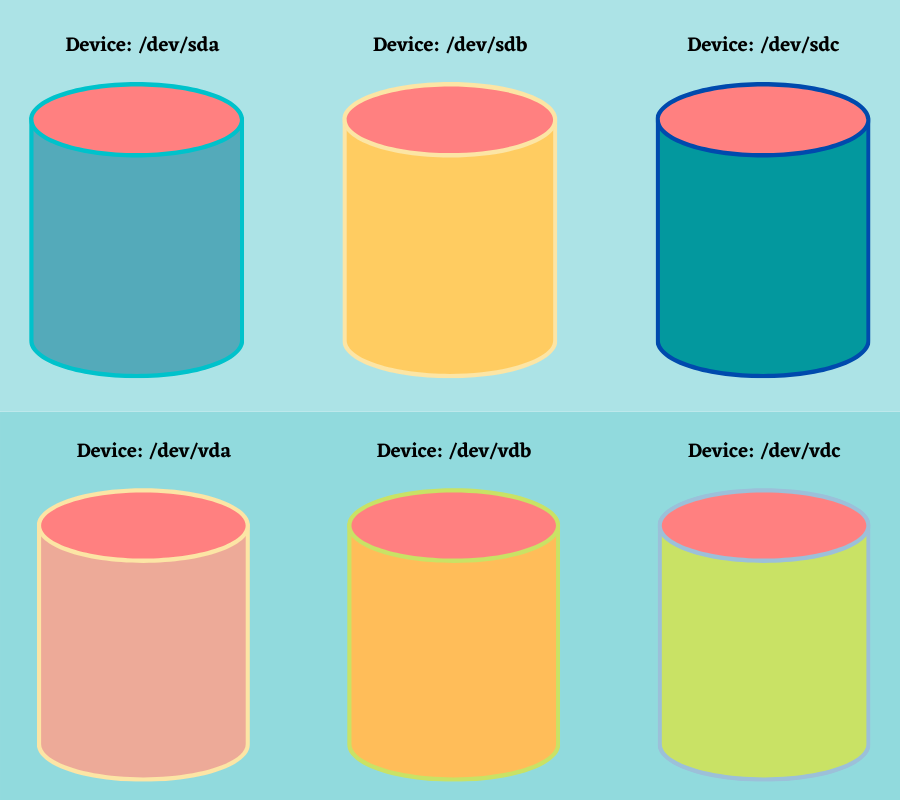
\includegraphics[scale=.38]{content/chapter8/images/name.png}
		\caption{Hard disk partitions}
		\label{HDD_naming}
	\end{figure}		
	\end{itemize}	
\newpage
\paragraph{Partition Names}
\begin{itemize}
	\item The partition are represented as numbers at the end of the HDD names.
	\item Eg: For HDD \textbf{"/dev/sda"}, partitions will be numbered as \textbf{/dev/sda1}, \textbf{/dev/sda2} and so on.
\end{itemize}
	\begin{figure}[h!]
	\centering
	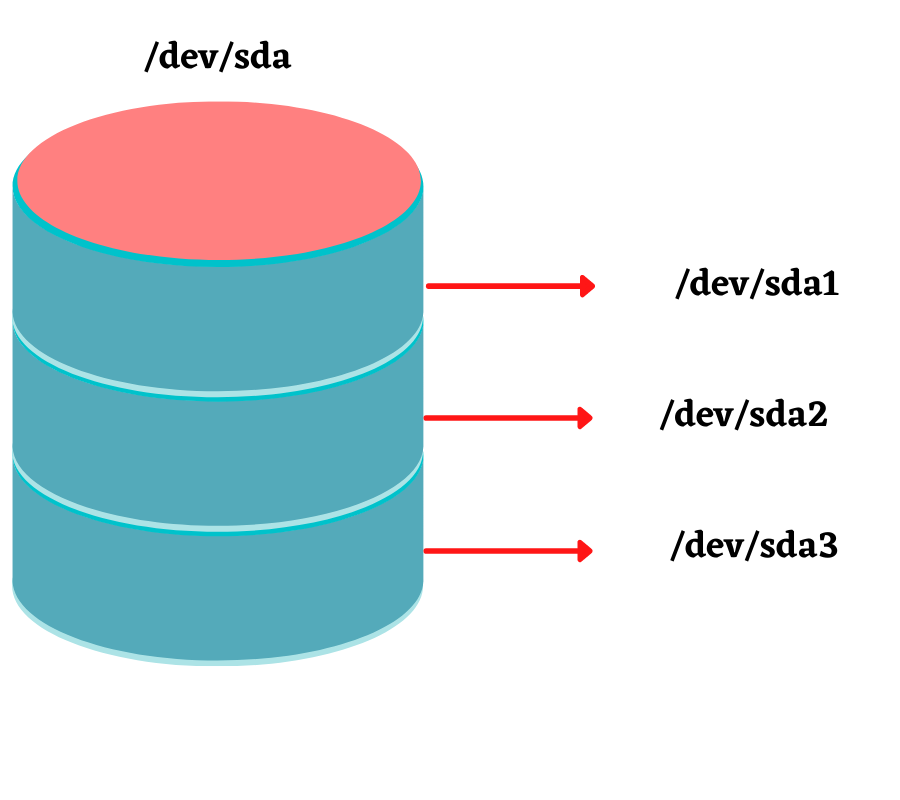
\includegraphics[scale=.38]{content/chapter8/images/partition_name.png}
	\caption{Partition names}
	\label{Partitions_naming}
\end{figure}		


\end{flushleft}
\newpage


